
%\maketile
\section{A few more Boolean problems}
\begin{example}
  Simplify the following Boolean expression:
  \[ f = x_1\bx_3 \bx_4 + x_2 \bx_3 \bx_4 + x_1 \bx_2 \bx_3 \]
\end{example}

\begin{example}
  Assume that a large room has three doors and that a switch near each door controls a light in the room. It has to be possible to turn the light on or off by changing the state of any one
  of the switches.\\
  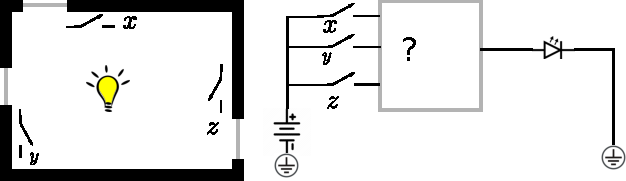
\includegraphics[width=\linewidth]{figures/design-a-3-way-light-switch.pdf}
\end{example}


\begin{prob}
A simple security system for two doors consists of a card reader and a keypad.

A person may open a particular door if he or she has a card containing the corresponding code and enters an authorized keypad code for that card. Note that card-code and keypad-code are different. The outputs from the card reader are given in the table below.


To unlock a door, a person must hold down the proper keys on the keypad and, then, insert the card in the reader. The authorized keypad code for door 1 is 10, and the authorized keypad code for door 2 is 11. If the card has an invalid code or if the wrong keypad code is entered, the alarm will ring when the card is inserted. If the correct keypad code is entered, the corresponding door will be unlocked when the card is inserted.

Design the logic circuit for this simple security system. Your circuit’s inputs will consist of a card code AB, and a keypad code CD. The circuit will have three outputs
XYZ (if X is 1, door 1 will be opened; if Y is 1, door 2 will be opened; if Z  1, the alarm will sound).

Find the minimal cost two-level circuit using K-maps for X, Y, Z. Provide the minimal cost. (It can be either of SOP/POS forms)\\

\includegraphics[width=0.5\linewidth]{figures/card-reader-keypad.png}%

\includegraphics[width=0.5\linewidth]{figures/card-reader-table.png}
\end{prob}
